\documentclass{beamer}
\mode<presentation>
\usepackage{amsmath,amssymb,mathtools}
\usepackage{textcomp}
\usepackage{gensymb}
\usepackage{adjustbox}
\usepackage{subcaption}
\usepackage{enumitem}
\usepackage{multicol}
\usepackage{listings}
\usepackage{url}
\usepackage{graphicx} % <-- needed for images
\def\UrlBreaks{\do\/\do-}

\usetheme{Boadilla}
\usecolortheme{lily}
\setbeamertemplate{footline}{
  \leavevmode%
  \hbox{%
  \begin{beamercolorbox}[wd=\paperwidth,ht=2ex,dp=1ex,right]{author in head/foot}%
    \insertframenumber{} / \inserttotalframenumber\hspace*{2ex}
  \end{beamercolorbox}}%
  \vskip0pt%
}
\setbeamertemplate{navigation symbols}{}

\lstset{
  frame=single,
  breaklines=true,
  columns=fullflexible,
  basicstyle=\ttfamily\tiny   % tiny font so code fits
}

\numberwithin{equation}{section}

% ---- your macros ----
\providecommand{\nCr}[2]{\,^{#1}C_{#2}}
\providecommand{\nPr}[2]{\,^{#1}P_{#2}}
\providecommand{\mbf}{\mathbf}
\providecommand{\pr}[1]{\ensuremath{\Pr\left(#1\right)}}
\providecommand{\qfunc}[1]{\ensuremath{Q\left(#1\right)}}
\providecommand{\sbrak}[1]{\ensuremath{{}\left[#1\right]}}
\providecommand{\lsbrak}[1]{\ensuremath{{}\left[#1\right.}}
\providecommand{\rsbrak}[1]{\ensuremath{\left.#1\right]}}
\providecommand{\brak}[1]{\ensuremath{\left(#1\right)}}
\providecommand{\lbrak}[1]{\ensuremath{\left(#1\right.}}
\providecommand{\rbrak}[1]{\ensuremath{\left.#1\right)}}
\providecommand{\cbrak}[1]{\ensuremath{\left\{#1\right\}}}
\providecommand{\lcbrak}[1]{\ensuremath{\left\{#1\right.}}
\providecommand{\rcbrak}[1]{\ensuremath{\left.#1\right\}}}
\theoremstyle{remark}
\newtheorem{rem}{Remark}
\newcommand{\sgn}{\mathop{\mathrm{sgn}}}
\providecommand{\abs}[1]{\left\vert#1\right\vert}
\providecommand{\res}[1]{\Res\displaylimits_{#1}}
\providecommand{\norm}[1]{\lVert#1\rVert}
\providecommand{\mtx}[1]{\mathbf{#1}}
\providecommand{\mean}[1]{E\left[ #1 \right]}
\providecommand{\fourier}{\overset{\mathcal{F}}{ \rightleftharpoons}}
\providecommand{\system}{\overset{\mathcal{H}}{ \longleftrightarrow}}
\providecommand{\dec}[2]{\ensuremath{\overset{#1}{\underset{#2}{\gtrless}}}}
\newcommand{\myvec}[1]{\ensuremath{\begin{pmatrix}#1\end{pmatrix}}}
\let\vec\mathbf

\title{MatGeo Presentation - Problem 6.3.4}
\author{EE25BTECH11064 - Yojit Manral}
\date{}

\begin{document}

\frame{\titlepage}
\begin{frame}{Question}
Find the shortest distance between the lines
\begin{align}
    \vec{r}&=(\vec{i}+2\vec{j}+\vec{k})+\kappa_1(\vec{i}-\vec{j}+\vec{k}) \\
    \vec{r}&=(2\vec{i}-\vec{j}-\vec{k})+\kappa_2(2\vec{i}+\vec{j}+2\vec{k})
\end{align}
\end{frame}

\begin{frame}{Solution}
$\longrightarrow$ The lines can be represented in vector form as
\begin{align}
    L_1 \equiv \vec{x} = \vec{A} + \kappa_1\vec{m_1} = \myvec{1\\2\\1} + \kappa_1\myvec{1\\-1\\1} \\
    L_2 \equiv \vec{x} = \vec{B} + \kappa_2\vec{m_2} = \myvec{2\\-1\\-1} + \kappa_2\myvec{2\\1\\2} 
\end{align}
$\rightarrow$ To check whether the given lines are skewed
\begin{align}
    \vec{M} = \myvec{\vec{m_1}&\vec{m_2}} = \myvec{1&2\\-1&1\\1&2}, &\vec{B}-\vec{A} = \myvec{1\\-3\\-2} \\
    \myvec{1&2&1\\-1&1&-3\\1&2&-2}\xrightarrow[R_3 \leftrightarrow R_3 - R_1]{R_2 \leftrightarrow R_2 + R_1}&\myvec{1&2&1\\0&3&-2\\0&0&-3} \\
    rank\myvec{\vec{M}&\vec{B}-\vec{A}} = 3 \implies& \text{ The given lines are skew}
\end{align}
\end{frame}

\begin{frame}{Solution}
$\longrightarrow$ Let $x_1(\mu_1)$ and $x_2(\mu_2)$ be the points closest to each other from the lines $L_1$ and $L_2$, respectively
\begin{align}
     \vec{x_1} = \vec{A} + \mu_1\vec{m_1} &&
     \vec{x_2} = \vec{B} + \mu_2\vec{m_2}
\end{align}
$\rightarrow$ Now, we have
\begin{align}
    (\vec{x_1}-\vec{x_2})^T\vec{m_1} = (\vec{x_1}-\vec{x_2})^T\vec{m_2} = 0 \\
    (\vec{x_1}-\vec{x_2})^T \myvec{\vec{m_1}&\vec{m_2}} = 0\\
    \vec{M}^T (\vec{x_1}-\vec{x_2}) = 0
\end{align}
$\rightarrow$ Using the \textit{least squares method}
\begin{align}
    \vec{x_1}-\vec{x_2} &= \vec{A}-\vec{B}+\myvec{\vec{m_1}&\vec{m_2}}\myvec{\mu_1\\-\mu_2} \\
    0 &= \vec{M}^T(\vec{A}-\vec{B})+\vec{M}^T\vec{M}\myvec{\mu_1\\-\mu_2} \\
    \vec{M}^T\vec{M}\vec{\mu} &= \vec{M}^T(\vec{B}-\vec{A}),\hspace{0.2cm} \vec{\mu} = \myvec{\mu_1\\-\mu_2}
\end{align}
\end{frame}

\begin{frame}{Solution}
$\longrightarrow$ To perform \textit{singular value decomposition}, we do the following eigen-decompositions
\begin{align}
    \vec{M}^T\vec{M} = \myvec{3&3\\3&9} = \vec{V}\vec{D_2}\vec{V}^T \\
    \vec{M}\vec{M}^T = \myvec{5&1&5\\1&2&1\\5&1&5} = \vec{U}\vec{D_1}\vec{U}^T 
\end{align}
$\rightarrow$ For $\vec{M}^T\vec{M}$, the characteristic polynomial is
\begin{align}
    char(\vec{M}^T\vec{M}) = \left|\begin{array}{cc}3-\lambda&3\\3&9-\lambda\end{array}\right| = \lambda^2 - 12\lambda + 18 \\
    \implies \lambda_1 = 6 + 3\sqrt{2}, \lambda_2 = 6 - 3\sqrt{2}
\end{align}
$\rightarrow$ For $\lambda_1$, the augmented matrix formed using the eigenvalue-eigenvector equation gives
\begin{align}
    \myvec{-3-3\sqrt{2}&3\\3&3-3\sqrt{2}}\xleftrightarrow{\text{which simplifies to}}\myvec{1&1-\sqrt{2}\\0&0}
\end{align}
\end{frame}

\begin{frame}{Solution}
\begin{align}
    \implies \vec{v_1} = \frac{1}{\sqrt{4-2\sqrt{2}}}\myvec{-1+\sqrt{2}\\1}
\end{align}
$\rightarrow$ For $\lambda_2$, the augmented matrix formed using the eigenvalue-eigenvector equation gives
\begin{align}
    \myvec{-3+3\sqrt{2}&3\\3&3+3\sqrt{2}}\xleftrightarrow{\text{which simplifies to}}\myvec{1&1+\sqrt{2}\\0&0} \\
    \implies \vec{v_2} = \frac{1}{\sqrt{4+2\sqrt{2}}}\myvec{-1-\sqrt{2}\\1}
\end{align}
$\rightarrow$ Using (15), we get
\begin{align}
    \vec{V} = \myvec{\vec{v_1}&\vec{v_2}} &= \myvec{\frac{-1+\sqrt{2}}{\sqrt{4-2\sqrt{2}}}&\frac{-1-\sqrt{2}}{\sqrt{4+2\sqrt{2}}} \\ \frac{1}{\sqrt{4-2\sqrt{2}}}&\frac{1}{\sqrt{4+2\sqrt{2}}}} \\
    \vec{D_2} &= \myvec{6+3\sqrt{2}&0\\0&6-3\sqrt{2}}
\end{align}
\end{frame}

\begin{frame}{Solution}
$\rightarrow$ For $\vec{M}\vec{M}^T$, the characteristic polynomial is
\begin{align}
    char(\vec{M}\vec{M}^T) = \left|\begin{array}{ccc}5-\lambda&1&5\\1&2-\lambda&1\\5&1&5-\lambda\end{array}\right| = \lambda(\lambda^2 - 12\lambda + 18) \\
    \implies \lambda_1 = 6 + 3\sqrt{2}, \lambda_2 = 6 - 3\sqrt{2}, \lambda_3 = 0
\end{align}
$\rightarrow$ For $\lambda_1$, the augmented matrix formed using the eigenvalue-eigenvector 
equation gives
\begin{align}
    \myvec{-1-3\sqrt{2}&1&5\\1&-4-3\sqrt{2}&1\\5&1&-1-3\sqrt{2}} \xleftrightarrow{\text{simplifies to}}\myvec{1&0&-1\\0&1&4-3\sqrt{2}\\0&0&0} \\
    \implies \vec{u_1} = \frac{1}{\sqrt{36-24\sqrt{2}}}\myvec{1\\-4+3\sqrt{2}\\1} = \frac{1}{\sqrt{12}}\myvec{1+\sqrt{2}\\2-\sqrt{2}\\1+\sqrt{2}}
\end{align}
\end{frame}

\begin{frame}{Solution}
$\rightarrow$ For $\lambda_2$, the augmented matrix formed using the eigenvalue-eigenvector equation gives
\begin{align}
    \myvec{-1+3\sqrt{2}&1&5\\1&-4+3\sqrt{2}&1\\5&1&-1+3\sqrt{2}}\xleftrightarrow{\text{simplifies to}}\myvec{1&0&-1\\0&1&4+3\sqrt{2}\\0&0&0} \\
    \implies \vec{u_2} = \frac{-1}{\sqrt{36+24\sqrt{2}}}\myvec{1\\-4-3\sqrt{2}\\1} = \frac{1}{\sqrt{12}}\myvec{1-\sqrt{2}\\2+\sqrt{2}\\1-\sqrt{2}}
\end{align}
$\rightarrow$ For $\lambda_3$, the augmented matrix formed using the eigenvalue-eigenvector equation gives
\begin{align}
    \myvec{5&1&5\\1&2&1\\5&1&5}\xleftrightarrow{\text{simplifies to}}\myvec{1&0&1\\0&1&0\\0&0&0}
\end{align}
\end{frame}

\begin{frame}{Solution}
\begin{align}
    \implies \vec{u_3} = \frac{1}{\sqrt{2}}\myvec{-1\\0\\1}
\end{align}
$\rightarrow$ Using (16), we get the following
\begin{align}
    \vec{U} = \myvec{\vec{u_1}&\vec{u_2}&\vec{u_3}} &= \myvec{\frac{1+\sqrt{2}}{\sqrt{12}}& \frac{1-\sqrt{2}}{\sqrt{12}}&-\frac{1}{\sqrt{2}}\\\frac{2-\sqrt{2}}{\sqrt{12}}&\frac{2+\sqrt{2}}{\sqrt{12}}&0\\\frac{1+\sqrt{2}}{\sqrt{12}}&\frac{1-\sqrt{2}}{\sqrt{12}}&\frac{1}{\sqrt{2}}} \\
    \implies \vec{U_R} &= \myvec{\frac{1+\sqrt{2}}{\sqrt{12}}&\frac{1-\sqrt{2}}{\sqrt{12}}\\\frac{2-\sqrt{2}}{\sqrt{12}}&\frac{2+\sqrt{2}}{\sqrt{12}}\\\frac{1+\sqrt{2}}{\sqrt{12}}&\frac{1-\sqrt{2}}{\sqrt{12}}} \\
    \vec{D_1} &= \myvec{6+3\sqrt{2}&0&0\\0&6-3\sqrt{2}&0\\0&0&0}
\end{align}
\end{frame}

\begin{frame}{Solution}
$\longrightarrow$ Then, for using \textit{singular value decomposition}, we define
\begin{align}
\vec{\Sigma} \triangleq \myvec{\sqrt{6+3\sqrt{2}}&0\\0&\sqrt{6-3\sqrt{2}}\\0&0} \implies
\vec{\Sigma_R} \triangleq \myvec{\sqrt{6+3\sqrt{2}}&0\\0&\sqrt{6-3\sqrt{2}}}
\end{align}
$\rightarrow$ Using \textit{singular value decomposition} and substituting in (14)
\begin{align}
    \vec{M} &= \vec{U_R}\vec{\Sigma_R}\vec{V}^T \\
    \vec{V}\vec{\Sigma_R}^T\vec{U_R}^T\vec{U_R}\vec{\Sigma_R}\vec{V}^T\vec{\mu} &= \vec{V}\vec{\Sigma_R}^T\vec{U_R}^T(\vec{B}-\vec{A}) \\
    \vec{V}\vec{\Sigma_R}^2\vec{V}^T\vec{\mu} &= \vec{V}\vec{\Sigma_R}\vec{U_R}^T(\vec{B}-\vec{A}) \\
    \vec{\mu} &= (\vec{V}\vec{\Sigma_R}^2\vec{V}^T)^{-1}\vec{V}\vec{\Sigma_R}\vec{U_R}^T(\vec{B}-\vec{A}) \\
    \vec{\mu} &= \vec{V}\vec{\Sigma_R}^{-2}\vec{V}^T\vec{V}\vec{\Sigma_R}\vec{U_R}^T(\vec{B}-\vec{A}) \\
    \vec{\mu} &= \vec{V}\vec{\Sigma_R}^{-1}\vec{U_R}^T(\vec{B}-\vec{A})
\end{align}
\end{frame}

\begin{frame}{Solution}
$\rightarrow$ Putting the required values in (42)
\begin{align}
    \vec{\mu} &= \myvec{\frac{-1+\sqrt{2}}{\sqrt{4-2\sqrt{2}}}&\frac{-1-\sqrt{2}}{\sqrt{4+2\sqrt{2}}}\\\frac{1}{\sqrt{4-2\sqrt{2}}}&\frac{1}{\sqrt{4+2\sqrt{2}}}} \myvec{\frac{1}{\sqrt{6+3\sqrt{2}}}&0\\0&\frac{1}{\sqrt{6-3\sqrt{2}}}} \notag \\
    &\hspace{2.5cm}\myvec{\frac{1+\sqrt{2}}{\sqrt{12}}&\frac{2-\sqrt{2}}{\sqrt{12}}&\frac{1+\sqrt{2}}{\sqrt{12}}\\\frac{1-\sqrt{2}}{\sqrt{12}}&\frac{2+\sqrt{2}}{\sqrt{12}}&\frac{1-\sqrt{2}}{\sqrt{12}}} \myvec{1\\-3\\-2} \\
    \myvec{\mu_1\\-\mu_2} &= \myvec{\frac{-1+\sqrt{2}}{\sqrt{12}}&\frac{-1-\sqrt{2}}{\sqrt{12}}\\\frac{1}{\sqrt{12}}&\frac{1}{\sqrt{12}}} \myvec{\frac{-7+2\sqrt{2}}{\sqrt{12}}\\\frac{-7-2\sqrt{2}}{\sqrt{12}}} = \myvec{11/6\\-7/6} \\
    \implies \myvec{\mu_1\\\mu_2} &= \myvec{11/6\\7/6}
\end{align}
\end{frame}

\begin{frame}{Solution}
$\longrightarrow$ This gives us the vector coordinates of $x_1$ and $x_2$, as
\begin{align}
\vec{x_1} = \myvec{1\\2\\1} + \brak{\frac{11}{6}}\myvec{1\\-1\\1} = \myvec{17/6\\1/6\\17/6} \\
\vec{x_2} = \myvec{2\\-1\\-1} + \brak{\frac{7}{6}}\myvec{2\\1\\2} = \myvec{26/6\\1/6\\8/6}
\end{align}
$\rightarrow$ And the least distance as
\begin{align}
    \norm{\vec{x_1}-\vec{x_2}} &= \left|\left|\myvec{-3/2\\0\\3/2}\right|\right| \\
    &=\frac{3\sqrt{2}}{2}
\end{align} 
\end{frame}

\begin{frame}{Solution}
\begin{figure}[h!]
   \centering
   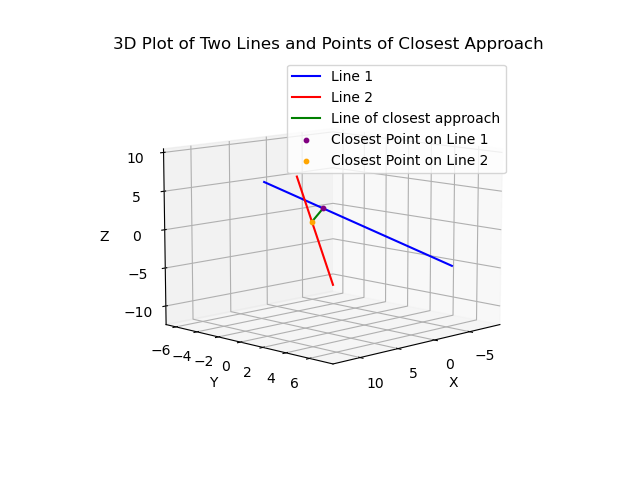
\includegraphics[width=0.85\linewidth]{figs/01.png}
   \caption{Plot of given lines and shortest distance between them}
   \label{Plot_1}
\end{figure}
\end{frame}
 % --------- CODE APPENDIX ---------
\section*{Appendix: Code}

% C program
\begin{frame}[fragile]{File: points.c}
\begin{lstlisting}[language=C]
#include <stdio.h>

int main() {
  FILE *fp;

  // -------------------
  // Question 6.3.4
  // -------------------


  fp = fopen("points.dat", "w");
  fprintf(fp, "%d,%d,%d\n", 1, 2, 1); // A
  fprintf(fp, "%d,%d,%d\n", 2, -1, -1); // B
  fprintf(fp, "%d,%d,%d\n", 1, -1, 1); // m1
  fprintf(fp, "%d,%d,%d\n", 2, 1, 2); // m2
  fprintf(fp, "%f,%f,%f\n", 17/6, 1/6, 17/6); // c1
  fprintf(fp, "%f,%f,%f\n", 26/6, 1/6, 8/6); // c2
  fclose(fp);
  return 0;
}
\end{lstlisting}
\end{frame}

% Python calling C
\begin{frame}[fragile]{File: call\_c.py}
\begin{lstlisting}[language=Python]
import subprocess

# Compile the C program
subprocess.run(["gcc", "points.c", "-o", "points"])

# Run the compiled C program
result = subprocess.run(["./points"], capture_output=True, text=True)

# Print the output from the C program
print(result.stdout)
\end{lstlisting}
\end{frame}

% Python plotting
\begin{frame}[fragile]{File: plot.py}
\begin{lstlisting}[language=Python]
import numpy as np
import matplotlib.pyplot as plt
from mpl_toolkits.mplot3d import Axes3D

# Define the lines with their parametric equations
# Define the parametric values for kappa_1 and kappa_2
kappa_1_vals = np.linspace(-5, 5, 50)
kappa_2_vals = np.linspace(-5, 5, 50)
# Parametric equations of the lines
r1 = np.array([1, 2, 1]) + kappa_1_vals[:, None] * np.array([1, -1, 1])
r2 = np.array([2, -1, -1]) + kappa_2_vals[:, None] * np.array([2, 1, 2])

# Plot the lines
fig = plt.figure()
ax = fig.add_subplot(111, projection='3d')
# Plot line 1
ax.plot(r1[:, 0], r1[:, 1], r1[:, 2], label='Line 1', color='blue')
# Plot line 2
ax.plot(r2[:, 0], r2[:, 1], r2[:, 2], label='Line 2', color='red')

# Points of closest approach on both lines
closest_point_1 = np.array([17/6,1/6,17/6])
closest_point_2 = np.array([26/6,1/6,8/6])
\end{lstlisting}
\end{frame}

% Python plotting
\begin{frame}[fragile]{File: plot.py}
\begin{lstlisting}[language=Python]
# Mark the vector along points of closest approach
closest_line_vals = np.linspace(0, 1, 10)
closest_line = np.array([17/6,1/6,17/6]) + closest_line_vals[:, None] * np.array([3/2,0,-3/2])
ax.plot(closest_line[:, 0], closest_line[:, 1], closest_line[:, 2], label='Line of closest approach', color='green')

# Mark the points of closest approach
ax.scatter(closest_point_1[0], closest_point_1[1], closest_point_1[2], color='purple', s=10, label='Closest Point on Line 1')
ax.scatter(closest_point_2[0], closest_point_2[1], closest_point_2[2], color='orange', s=10, label='Closest Point on Line 2')

# Labels and title
ax.set_xlabel('X')
ax.set_ylabel('Y')
ax.set_zlabel('Z')
ax.set_title('3D Plot of Two Lines and Points of Closest Approach')

# Set the camera angle
ax.view_init(elev=10, azim=45)

# Show the plot
ax.legend()
plt.show()
\end{lstlisting}
\end{frame}

\end{document}
